Let us consider a system
\begin{eqnarray}
%\begin{array}{c}
{\cal L} 
&=&
{\cal L_{\psi}} + {\cal L_{\phi}}  - g \phi \overline{\psi} \psi\,,
\vspace{2mm}
\\
{\cal L_{\psi}} 
&=&
\overline{\psi} (
i \slashed{\partial} - m ) \psi
\,,
\hspace{5mm}
{\cal L_{\phi}} 
=
\frac{1}{2} (\partial_\mu \phi)^2 
-
\frac{1}{2} \mu^2 \phi^2
%\end{array}
\label{eqn:DirYkwLagDens}
\end{eqnarray}
with a Dirac nucleon field $\psi$ with the mass $m$
and a scalar pion field $\phi$ with the mass $\mu$.
The interaction term ${\cal L}_{int} = -g \phi \overline{\psi} \psi$ shows they interact
each other through the Yukawa coupling.

\bigskip

\noindent
\underline{$NN \to NN$}\\
Initial and final states:
\begin{eqnarray}
\begin{array}{l}
\ketend i \ket
= c_{r_a}^\dagger (\bld{p}_a) c_{r_b}^\dagger (\bld{p}_b) \ketend 0 \ket
\rightdef \ketend N_a, N_b \ket
\vspace{2mm}
\\
\ketend f \ket
= c_{r_1}^\dagger (\bld{p}_1) c_{r_2}^\dagger (\bld{p}_2) \ketend 0 \ket
\rightdef \ketend N_1, N_2 \ket
\end{array}
\label{eqn:IniFinNNtoNN}
\end{eqnarray}
S-matrix element of the lowest order
\begin{eqnarray}
\bra f \braend S^{(2)} \ketend i \ket
&=&
\frac{(-ig)^2}{2} \int d^4 x_1' d^4 x_2'
\bra N_2 N_1 \braend
T[\normalprod{\phi_{1'} \overline{\psi}_{1'} \psi_{1'}}
\normalprod{\phi_{2'} \overline{\psi}_{2'} \psi_{2'}}
]
\ketend N_a N_b \ket
\nonumber\\
%&& +\cdots
&=&
\frac{(-ig)^2}{2} \int d^4 x_1' d^4 x_2'
\Delta_F(x_1' - x_2')
\bra N_2 N_1 \braend
T[\normalprod{\overline{\psi}_{1'} \psi_{1'}}
\normalprod{ \overline{\psi}_{2'} \psi_{2'}}
]
\ketend N_a N_b \ket
\nonumber\\
\label{eqn:DiracNNNNS2formula}
\end{eqnarray}
Arguments of fields are indicated by suffices.
Wick's theorem reads
\begin{eqnarray}
%&&
\bra N_2 N_1 \braend
T[\normalprod{\overline{\psi}_{1'} \psi_{1'}}
\normalprod{ \overline{\psi}_{2'} \psi_{2'}}
]
\ketend N_a N_b \ket
%\nonumber\\
%&&
=
\bra N_2 N_1 \braend
\normalprod{\overline{\psi}_{1'} \psi_{1'}
 \overline{\psi}_{2'} \psi_{2'}
}
\ketend N_a N_b \ket
\label{eqn:DiracNNNNsand}
\end{eqnarray}
Decompose Dirac fields as
\begin{eqnarray}
\psi = \psi^{(+)}(c) + \psi^{(-)}(d^\dagger)\,,
\hspace{3mm}
\overline{\psi} = \overline{\psi^{(+)}}(c^\dagger) + \overline{\psi^{(-)}}(d)
\label{eqn:DiracSpDecomp}
\end{eqnarray}
where arguments should be understood just as symbols to remember definitions
of decomposed fields given below:
\begin{eqnarray}
\left\{
\begin{array}{l}
\displaystyle
\psi^{(+)}_{l \alpha} (c)
=
\int \frac{d^3 \bld{p}}{\sqrt{(2\pi)^3} 2 p^0}
\sum_{r=1,2}
c_r (\bld{p}) u_\alpha^{(r)} (\bld{p}) e^{-ipx_l}
\;\rightdef
c_{l (r, p)} u_\alpha^{(r,p)}
\vspace{2mm}
\\
\displaystyle
\overline{\psi^{(+)}}_{l \alpha} (c^\dagger)
=
\int \frac{d^3 \bld{p}}{\sqrt{(2\pi)^3} 2 p^0}
\sum_{r=1,2}
c_r^\dagger (\bld{p}) \bar{u}_\alpha^{(r)} (\bld{p}) e^{ipx_l}
\;\rightdef
c^\dagger_{l (r, p)} \bar{u}_\alpha^{(r,p)}
\vspace{2mm}
\\
\displaystyle
\psi^{(-)}_{l \alpha} (d^\dagger)
=
\int \frac{d^3 \bld{p}}{\sqrt{(2\pi)^3} 2 p^0}
\sum_{r=1,2}
d^\dagger_r (\bld{p}) v_\alpha^{(r)} (\bld{p}) e^{ipx_l}
\;\rightdef
d^\dagger_{l (r, p)} v_\alpha^{(r,p)}
\vspace{2mm}
\\
\displaystyle
\overline{\psi^{(-)}}_{l \alpha} (d)
=
\int \frac{d^3 \bld{p}}{\sqrt{(2\pi)^3} 2 p^0}
\sum_{r=1,2}
d_r (\bld{p}) \bar{v}_\alpha^{(r)} (\bld{p}) e^{-ipx_l}
\;\rightdef
d_{l (r, p)} \bar{v}_\alpha^{(r,p)}
\end{array}
\right.
\label{eqn:DiracFDecompDef}
\end{eqnarray}
Indexes of spinors are explicitly shown. 
Last equations in each line define symbols to abbreviate 
expressions in the left hand side.
Substituting the decomposition 
(\ref{eqn:DiracSpDecomp}) in
Eq. (\ref{eqn:DiracNNNNsand}), it becomes
\begin{eqnarray}
&&\bra N_2 N_1 \braend
\normalprod{\overline{\psi}_{1' \alpha} \psi_{1' \alpha}
 \overline{\psi}_{2' \beta} \psi_{2' \beta}
}
\ketend N_a N_b \ket
\nonumber\\
&&=
\bra N_2 N_1 \braend
\normalprod{\overline{\psi^{(+)}}_{1' \alpha} \psi^{(+)}_{1' \alpha}
 \overline{\psi^{(+)}}_{2' \beta} \psi^{(+)}_{2' \beta}
}
\ketend N_a N_b \ket
\nonumber\\
&&=
\bra N_2 N_1 \braend
\overline{\psi^{(+)}}_{1' \alpha}  \overline{\psi^{(+)}}_{2' \beta} 
\psi^{(+)}_{2' \beta} \psi^{(+)}_{1' \alpha}
\ketend N_a N_b \ket
\nonumber\\
&&=
\bra 0 \braend c_{2} c_1 \left\{
c^\dagger_{1'(1')} c^\dagger_{2'(2')} c_{2'(b')} c_{1'(a')}
\right\}
c^\dagger_{a} c^\dagger_{b} \ketend 0 \ket
\bar{u}_\alpha^{(1')} \bar{u}_\beta^{(2')} u_\beta^{(b')}u_\alpha^{(a')}
\,,
\nonumber\\
\label{eqn:DirNNNNsandIntermed}
\end{eqnarray}
In the last expression, we have used abbreviations
\begin{eqnarray}
\begin{array}{l}
c_1 = c_{r_1}(\bld{p}_1)\,
\vspace{2mm}
\\
c_{1' (a')} = c_{1'(r_{a'} p_{a'})}\,,
\hspace{3mm}
u_\alpha^{(a')} = u_\alpha^{(r_{a'}, p_{a'})}
\end{array}
\end{eqnarray}
%------------------------------------------
\begin{eqnarray}
(\ref{eqn:DirNNNNsandIntermed}) \bra 0 \braend \cdots  \ketend 0 \ket
&=&
\bra 0 \braend c_{2}
\left\{
[ c_1, c^\dagger_{1'(1')}]_+ - c^\dagger_{1'(1')} c_1
\right\}
 c^\dagger_{2'(2')} 
 \nonumber\\
 &&
 c_{2'(b')} 
\left\{
[c_{1'(a')}, c^\dagger_{a} ]_+ - c^\dagger_{a} c_{1'(a')}
\right\}
c^\dagger_{b} \ketend 0 \ket
 \nonumber\\
 &=&
\bra 0 \braend 
\left\{
[ c_1, c^\dagger_{1'(1')}]_+
[c_{2}, c^\dagger_{2'(2')} ]_+
-
[c_{2},  c^\dagger_{1'(1')}]_+ 
[c_1, c^\dagger_{2'(2')} ]_+
\right\}
 \nonumber\\
 &&
\left\{
[c_{1'(a')}, c^\dagger_{a} ]_+ 
[ c_{2'(b')}, c^\dagger_{b}]_+ 
- 
[ c_{2'(b')}, c^\dagger_{a}]_+ 
[ c_{1'(a')}, c^\dagger_{b}]_+ 
\right\}
 \ketend 0 \ket
 \nonumber\\ 
\label{eqn:DirNNNNvacsandInterm}
\end{eqnarray}
where $[\cdots]_+$ stands for anti-commutator. 
We have, for instance
\begin{eqnarray}
\begin{array}{l}
\displaystyle
[c_1, c^\dagger_{1' (a') }]_+
=
\frac{1}{\sqrt{(2\pi)^3}}
\sum_{(a')} \delta_{(a') 1} e^{i p_{a'} x_{1'}} \times
\\
\displaystyle
[ c_{1'(a')}, c^\dagger_{b}]_+ 
=
\frac{1}{\sqrt{(2\pi)^3}}
\sum_{(a')} \delta_{(a') b} e^{-i p_{a'} x_{1'} } \times
\vspace{2mm}
\end{array}
\end{eqnarray}
where
\begin{eqnarray}
\sum_{(a')} \delta_{(a') a} \times
\leftdef
\int d^3 \bld{p}_{a'} \sum_{r_{a'}}
\delta^3(\bld{p}_{a'} - \bld{p}_a) \delta_{r_{a'} r_a} \times
\end{eqnarray}
and the multiplication at the end means
factors behind are involved in the summation. 
\begin{eqnarray}
(\ref{eqn:DirNNNNsandIntermed}) 
&=&
\frac{1}{(2\pi)^6}
\sum_{(1')(2')(a')(b')}
\left\{
(
\delta_{1(1')}\delta_{2(2')}
-
\delta_{2(1')}\delta_{1(2')}
)
(
\delta_{(a')a}\delta_{(b')b}
-
\delta_{(b')a}\delta_{(a')b}
)
\right\}
 \times
\nonumber\\
&&
e^{i(p_{1'} x_{1'} + p_{2'} x_{2'}  - p_{a'} x_{1'} - p_{b'} x_{2'}    )}
\bar{u}_\alpha^{(1')} u_\alpha^{(a')} \bar{u}_\beta^{(2')} u_\beta^{(b')}
\label{eqn:DirNNNNabbamp}
\end{eqnarray}
%In Eq. (\ref{eqn:DiracNNNNS2formula}), one may exchage $x_1'$ and $x_2'$ and
Remembering that $\Delta_F$ is an even function,
\begin{eqnarray}
S_{fi}^{(2)}
&=&
\frac{(-ig)^2}{2}
\int d^4 x_1' d^4 x_2' \Delta_F(x_1' - x_2')
\frac{1}{(2\pi)^6}
\sum_{(1')(2')(a')(b')}
\nonumber\\
&&
\left\{
\delta_{(1')1}\delta_{(2')2}
\delta_{(a')a}\delta_{(b')b}
+
\delta_{2(1')}\delta_{1(2')}
\delta_{(a')b}\delta_{(b')a}
%\right.
%\nonumber\\
%&&
%\left.
-
\delta_{(1')1}\delta_{(2')2}
\delta_{(a')b}\delta_{(b')a}
-
\delta_{2(1')}\delta_{1(2')}
\delta_{(a')a}\delta_{(b')b}
\right\}
\nonumber\\
&&
e^{i(p_{1'} x_{1'} + p_{2'} x_{2'}  - p_{a'} x_{1'} - p_{b'} x_{2'}    )}
\bar{u}_\alpha^{(1')} u_\alpha^{(a')} \bar{u}_\beta^{(2')} u_\beta^{(b')}
\nonumber\\
&=&
\frac{(-ig)^2}{(2\pi)^6}
\int d^4 x_1' d^4 x_2' \Delta_F(x_1' - x_2')
\sum_{(1')(2')(a')(b')}
\left\{
\delta_{(1')1}\delta_{(2')2}
\delta_{(a')a}\delta_{(b')b}
-
\delta_{2(1')}\delta_{1(2')}
\delta_{(a')a}\delta_{(b')b}
\right\}
\nonumber\\
&&
e^{i(p_{1'} x_{1'} + p_{2'} x_{2'}  - p_{a'} x_{1'} - p_{b'} x_{2'}    )}
\bar{u}_\alpha^{(1')} u_\alpha^{(a')} \bar{u}_\beta^{(2')} u_\beta^{(b')}
\nonumber\\
&=&
\frac{(-ig)^2}{(2\pi)^6}
\int d^4 x_1' d^4 x_2' \Delta_F(x_1' - x_2')
\left\{
e^{i(p_{1} x_{1'} + p_{2} x_{2'}  - p_{a} x_{1'} - p_{b} x_{2'} )}
\bar{u}_\alpha^{(1)} u_\alpha^{(a)} \bar{u}_\beta^{(2)} u_\beta^{(b)}
\right.
\nonumber\\
&&
\hspace{50mm}
\left.
-
e^{i(p_{2} x_{1'} + p_{1} x_{2'}  - p_{a} x_{1'} - p_{b} x_{2'} )}
\bar{u}_\alpha^{(2)} u_\alpha^{(a)} \bar{u}_\beta^{(1)} u_\beta^{(b)}
\right\}
\nonumber\\
&=&
\frac{(-ig)^2}{(2\pi)^6}
\int d^4 k
\frac{i (2\pi)^4}{k^2 - \mu^2 + i\epsilon}
\left\{
\delta^4(p_1 - p_a - k) \delta^4(p_2 - p_b + k)
\bar{u}_\alpha^{(1)} u_\alpha^{(a)} \bar{u}_\beta^{(2)} u_\beta^{(b)}
\right.
\nonumber\\
&&
\hspace{40mm}
\left.
-
\delta^4(p_2 - p_a - k) \delta^4(p_1 - p_b + k)
\bar{u}_\alpha^{(2)} u_\alpha^{(a)} \bar{u}_\beta^{(1)} u_\beta^{(b)}
\right\}
\nonumber\\
&=&
\nonumber\\
&&
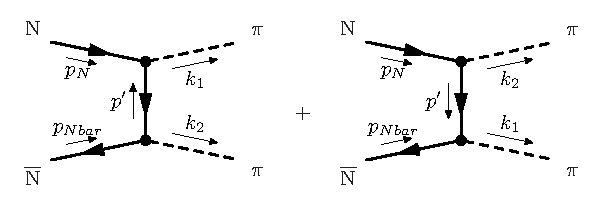
\includegraphics{\feynmfdirectory/05DirNN2NN/Smtrx2.eps}
\nonumber\\
&=&
i(2\pi)^4 \delta^4(P_f - P_i)
\frac{(-ig)^2}{(2\pi)^6}
\left\{
\frac{\bar{u}_\alpha^{(1)} u_\alpha^{(a)} \bar{u}_\beta^{(2)} u_\beta^{(b)}}
{(p_1 - p_a)^2 - \mu^2 + i\epsilon}
-
\frac{\bar{u}_\alpha^{(2)} u_\alpha^{(a)} \bar{u}_\beta^{(1)} u_\beta^{(b)}}
{(p_2 - p_a)^2 - \mu^2 + i\epsilon}
\right\}
%\nonumber\\
\label{eqn:DirYukS2Feynm}
\end{eqnarray}

\begin{eqnarray}
T^{(2)}_{fi} 
=
\frac{(-ig)^2}{(2\pi)^6}
\left\{
\frac{\bar{u}_\alpha^{(1)} u_\alpha^{(a)} \bar{u}_\beta^{(2)} u_\beta^{(b)}}
{(p_1 - p_a)^2 - \mu^2 + i\epsilon}
-
\frac{\bar{u}_\alpha^{(2)} u_\alpha^{(a)} \bar{u}_\beta^{(1)} u_\beta^{(b)}}
{(p_2 - p_a)^2 - \mu^2 + i\epsilon}
\right\}
\label{eqn:DirYukT2Feynm}
\end{eqnarray}
Though the meaning of our short-hand notations are stated before, 
we write here again that $u^{(1)}$ in the above equation, for instance,
stands for $u^{r_1}(\bld{p}_1)$.

%\bigskip

\newpage
\noindent
{\bf Feynman rules for Dirac fermions}\\
\begin{enumerate}
\item
For each incoming (outgoing) fermion with momentum $\bld{p}$ and polarization $r$, 
associate $u^{(r)}(\bld{p})/\sqrt{(2\pi)^3}$ ($\bar{u}^{(r)}(\bld{p})/\sqrt{(2\pi)^3}$).
For each incoming (outgoing) anti-fermion, associate $\bar{v}^{(r)}(\bld{p})/\sqrt{(2\pi)^3}$ 
(${v}^{(r)}(\bld{p})/\sqrt{(2\pi)^3}$).

\item
To each vartex, associate a factor $(-ig) (2\pi)^4 \delta^4(\sum_{in} p_{in})$.

\item
For each internal fermion line, write a factor of
\begin{eqnarray}
\int \frac{d^4 p'}{(2\pi)^4}
\frac{i (\slashed{p'} + m )}{p^{'2} - m^2 + i\epsilon}
\end{eqnarray}
\end{enumerate}
